
\documentclass{sig-alternate}
%%\documentclass{article} %% hevea
%%\usepackage[utf8]{inputenc} %% hevea


\usepackage{hyperref}

%% url
\usepackage{url}
%% maths
\usepackage{bm}
%\usepackage[cmex10]{amsmath}
%\usepackage{amsfonts}
%\usepackage{amssymb}
%% algorithms
\usepackage{algorithm}
\usepackage{algorithmicx}
\usepackage{algpseudocode}
%% images
\usepackage{graphicx}
\usepackage{subfig}
%% inparaenum
\usepackage{paralist}
%% tables
\usepackage{booktabs}
\usepackage{multirow}
%% figures
\usepackage{tikz}
\usetikzlibrary{decorations.pathreplacing,plotmarks,shapes}
%% transform eps in pdf crossplateform
\usepackage{epstopdf}
\usepackage{epsfig}

\usepackage{enumitem}
\usepackage{xspace}

\newcommand{\TODO}[1]{\textcolor{red}{#1}}
\newcommand{\LSEQ}[0]{\textsc{LSeq}\xspace}
\newcommand{\CRATE}[0]{\textsc{Crate}\xspace}
\newcommand{\SPRAY}[0]{\textsc{Spray}\xspace}


\newcounter{example}
\setcounter{example}{0}
\newcommand{\EXAMPLE}[0]{\stepcounter{example}\the\value{example}}

%%paralist
%\renewcommand*\descriptionlabel[1]{%
%\scshape #1}
%\renewcommand\paradescriptionlabel[1]{%
%\scshape #1}

%%%%%%%%%%%%%%%%%%%%%%%%%%%%%%%%%%%%%%%%%%%%%%%%%%%%%%%%%%%%%%%%%%%%%%%%%%%%%%%
%%%%%%%%%%%%%%%%%%%%%%%%%%%%%%%%%%%%%%%%%%%%%%%%%%%%%%%%%%%%%%%%%%%%%%%%%%%%%%%
%%%%%%%%%%%%%%%%%%%%%%%%%%%%%%%%%%%%%%%%%%%%%%%%%%%%%%%%%%%%%%%%%%%%%%%%%%%%%%%

\begin{document}

\title{CRATE: a Scalable Decentralized Real-Time Editor}

\numberofauthors{1}
\author{
     \alignauthor Brice N\'edelec, Pascal Molli, Achour Mostefaoui\\
     \affaddr{LINA, 2 rue de la Houssini\`ere}\\
     \affaddr{BP92208, 44322 Nantes Cedex 03}\\
     \email{first.last@univ-nantes.fr}
}

\maketitle


Google Docs made real-time editing in browsers easy for millions of
users. However, Google mediates real-time editing sessions with
central servers raising issues on privacy, censorship, economic
intelligence. It also raises scalability issues in term of number of
participants.  Despite that small groups currently constitute the main
range of users, events such as massive online lectures, TV shows,
conferences gather larger groups.  Google Docs supports large groups
but only the first fifty users can edit, next users have their rights
limited to document reading. We think that real-time editors should allow
editing at anytime and anywhere, whatever the number of
participants.

%% In this paper we focus on building a real-time editor that supports privacy
%% and that adapts \TODO{gently} from small groups to large groups

Decentralized real-time editors~\cite{oster2006data, sun1998operational,
  sun2009contextbased} do not require intermediate servers and by the same
settle privacy issues. However, scalability issues remain.  Addressing
scalability requires finding a good trade-off between communication, space and
time complexities. Achieving a sublinear communication complexity compared to
the number of participants is crucial for supporting large groups.

%% But consistency maintenance of documents requires each message to piggyback
%% additional information which greatly impacts the communication complexity.

To provide availability and responsiveness of documents, real-time editors use
the optimistic replication. As such, each user creates a local copy of the
document and directly performs her modification on it. Changes are broadcast to
all replica owners where they are integrated. Strong eventual consistency states
that replicas integrating an identical set of operations converge to an
equivalent state, i.e., users read a same document.

Decentralized algorithms of Operational
Transformation~\cite{sun2009contextbased} (OT) require piggybacking a
state or a context vector in order to detect concurrent
operations. Unfortunately, state vectors grow linearly compared to the
number of members that ever participated in the authoring. Hence,
these approaches behave great with stable small groups of users, but
poorly scale to highly dynamic large group of users and high latency.

Conflict-Free Replicated Data Types~\cite{shapiro2011comprehensive}
(CRDTs) avoid paying the price of concurrency detection by providing
commutative operations. However, they require to piggyback unique and
immutable identifiers to every operation broadcast on the network. The
size of this identifier is the key for the communication complexity
and consequently the scalability of the approach. Two classes of CRDTs
designed for sequences exist:
\begin{itemize}
\item CRDTs such as WOOT~\cite{oster2006data} piggyback a
  constant-size identifer which is optimal. However, it requires to
  keep tombstones ie. mark removed elements from the structure and
  hide them from the users. A document may appear empty while storing
  thousands of unnecessary elements. Tombstones degrades time
  complexity for integrating operations and can make the real-time editor
  unusable. Removing tombstones require a costly garbage collecting
  algorithms that can hardly be deployed in such context.
\item CRDTs such as Logoot~\cite{weiss2010logootundo} do not require tombtones but
  piggyback variable size identifiers. Depending on the identifier
  allocation strategy, they may grow linearly with the document
  size and degrades quickly the communication complexity. The
  replicated structure eventually need an unaffordable balancing
  mechanism.

  The allocation strategy \LSEQ~\cite{nedelec2013concurrency} aims to
  avoid such balancing mechanism by sublinearly upper-bounding the
  space complexity of its identifiers. It conjectured a
  polylogarithmic growth of the identifiers size
  $\mathcal{O}((\log d)^2)$ where $d$ is the document
  size. %Experiments empirically confirmed the conjecture.
\end{itemize}

The contributions of  this paper are threefold:
\begin{itemize}
\item Compared to previous work~\cite{nedelec2013concurrency} , we
  demonstrate the upper bounds on space and time complexities of
  LSeq. This result opens the way for building decentralized and
  scalable real-time editors. % we thoroughly analyze the \LSEQ's
  % complexity in time, space and communication. In particular, we
  % isolate three editing behaviors: left-to-right, right-to-left, and
  % random -- real-life editing being a composition of these
  % three. \LSEQ sacrifices on its worst-case complexity which
  % \TODO{rarely} happens to improve the identifiers size of common
  % editing behaviors. They become polylogarithmically upper-bounded
  % compared to the document size.
\item We describe all the outlines to develop a distributed
  collaborative editor for massive editing of large documents.
\item We built a real-time decentralized editor running in web
  browser\footnote{\url{https://github.com/Chat-Wane/CRATE}}. In the Grid'5000
  testbed, we launched an editing session involving up till 600 connected
  browsers. The resulting documents reach millions of
  characters. Figure~\ref{fig:traffic} shows the result of the experiment. We
  observe that the traffic generated grows following $\ln N (\log d)^2$ where
  $N$ is the network size, $\ln N$ is a multiplicative factor brought by
  scalable broadcast~\cite{nedelec2015spray}, $d$ is the document size, and $(\log d)^2$ is
  brought by the messages piggybacking \LSEQ's identifiers.
\end{itemize}

\begin{figure}
  \centering
  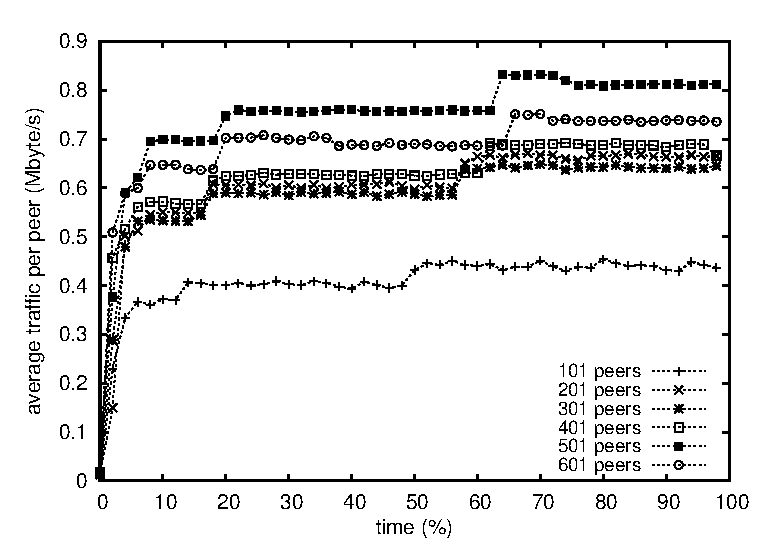
\includegraphics[width=0.8\textwidth]{img/traffic.eps}
  \caption{\label{fig:traffic} Traffic generated by editing sessions of
    various size.}
\end{figure}

%%% Local Variables: 
%%% mode: latex
%%% TeX-master: "../paper"
%%% End: 


\keywords{
Document authoring, distributed collaborative editing, optimistic replication,
polylog sequence encoding, Conflict-free Replicated Data Types}

%%% Local Variables: 
%%% mode: plain-tex
%%% TeX-master: "../paper"
%%% End: 



\section{Introduction}

Google Docs or Etherpad allow millions of users to start and access real-time
editing sessions very easily by the mean of URLs in web browsers. Yet, such
editors require collaboration providers to setup servers and enable
collaboration. It implies issues in privacy, censorship, and economic
intelligence. It also implies scalability issues in term of number of
participants. Despite that current editors limit \emph{de facto} the groups
size, emerging contexts (e.g. massive online courses, conferences, TV-shows)
expose the needs of larger collaboration groups.  For instance, writing notes on
Google Docs is possible uptill fifty users. Next users have their rights limited
to the reading of the document.

Decentralized real-time editors~\cite{oster2006data, sun1998operational,
  sun2009contextbased} do not require intermediate servers and by the same solve
privacy-related issues. However, scalability issues remain.  Addressing
scalability issues requires finding a good trade-off between communication,
space and time complexities. Such trade-off mainly consists in a sublinear
communication complexity compared to the editing session size. While the
transmission of operations requires at least a multiplicative factor
logarithmically scaling compared to the network size, maintaining consistency
requires piggybacking additional metadata the complexity of which must be
carefully studied.

Decentralized algorithms that belong to operational
transformation~\cite{sun2009contextbased} approach require piggybacking a state
vector in order to detect concurrent operations. Unfortunately, state vectors
grow linearly compared to the number of members that ever participated in the
authoring.

Conflict-Free Replicated Data Types~\cite{shapiro2011comprehensive} (CRDTs) such
as WOOT~\cite{oster2006data} piggyback a constant-size identifier which is
optimal. Nonetheless, their local space complexity grows monotonically which
eventually leads to the need of an unaffordable garbage collecting. Other
algorithms~\cite{preguica2009commutative, weiss2010logootundo} limit their local
space consumption. Nevertheless, they piggyback variable-size identifiers that
can grow linearly compared to the document size. In such case, they eventually
need to run a costly consensus algorithm to rebalance
documents~\cite{zawirski2011asynchronous}. Finally, the \LSEQ
algorithm~\cite{nedelec2013concurrency} aims to avoid such consensus by
sublinearly upper-bounding the space complexity of its identifiers. \TODO{It
  conjectured that identifiers can be bounded to the $log(s)^2$ where $s$ is the
  size of shared document.}

In this paper, we propose \CRATE, a scalable real-time editor that runs on a
network of browsers. \CRATE relies on WebRTC and browser-to-browser
communication to provide an easy access for end-users. Compared to
state-of-the-art, it presents a different tradeoff which balances the load
between space, time, and communication complexities. The contributions of this
paper are threefold:
\begin{itemize}
\item Compared to previous work~\cite{nedelec2013lseq}, we demonstrate the upper
  bounds on space and time complexities of \LSEQ. In addition to which we
  provide the communication complexity of \CRATE. We shows the balance in these
  dimensions and we position it in relation to state-of-the-art.
\item We describe \CRATE's internal components. In particular, we detail \LSEQ
  that manages the shared document, and \SPRAY that creates the network of
  browsers. Our Javascript implementation of \CRATE runs directly in browsers
  without any plugins.
\item We conducted experimental studies to validate the complexities of
  \CRATE. The experiments took place in the Grid'5000 testbed and involved
  uptill $600$ real web browsers opened to edit a shared document. At a rate of
  100 insertions per seconds, the document size reached above 1 million
  characters. As expected, we observed a logarithmic growth of the traffic
  compared to the number of participants, and a polylogarithmic growth of the
  traffic compared to the size of the document.
\end{itemize}

The remainder of this paper is organized as follows:
Section~\ref{sec:relatedwork} reviews the related work with an emphasis on the
complexity tradeoff proposed by other approaches. Section~\ref{sec:proposal}
follows with a description of \CRATE and its core
components. Section~\ref{sec:experiments} highlights the scalability of \CRATE
while validating the complexity analysis of \LSEQ and \SPRAY. Finally,
Section~\ref{sec:conclusion} concludes the paper and discusses about
perspectives.

%%% Local Variables: 
%%% mode: latex
%%% TeX-master: "../paper"
%%% End: 

\section{Related Work}
\label{sec:relatedwork}

\begin{table*}
  \centering
  

\begin{tabular}{@{}lccccccc@{}}
  \toprule
  & \multicolumn{4}{c}{\textsc{time}} & \multicolumn{2}{c}{\textsc{space}} & \textsc{communication} \\ \cmidrule{2-8}
  & \multicolumn{2}{c}{\textsc{local}} & \multicolumn{2}{c}{\textsc{remote}} & & & \\ \cmidrule{2-5}
  & \textsc{ins} & \textsc{del} & \textsc{ins} & \textsc{del} & \textsc{sequence} & \textsc{causality} & \textsc{message} \\ \midrule
  SOCT2/TTF & $O()$ & $O()$ & $O()$ & $O()$ & $O()$ & $O()$ & $O()$ \\ \midrule
  \TODO{COT-DO} & $O()$ & $O()$ & $O()$ & $O()$ & $O()$ & $O()$ & $O()$ \\ \midrule
  WOOT & $O()$ & $O()$ & $O()$ & $O()$ & $O()$ & $O()$ & $O()$ \\ \midrule
  WOOTO & $O()$ & $O()$ & $O()$ & $O()$ & $O()$ & $O()$ & $O()$ \\ \midrule
  WOOTH & $O()$ & $O()$ & $O()$ & $O()$ & $O()$ & $O()$ & $O()$ \\ \midrule
  RGA & $O()$ & $O()$ & $O()$ & $O()$ & $O()$ & $O()$ & $O()$ \\ \midrule
  \TODO{SW} & $O()$ & $O()$ & $O()$ & $O()$ & $O()$ & $O()$ & $O()$ \\ \midrule
  \TODO{PPS} & $O()$ & $O()$ & $O()$ & $O()$ & $O()$ & $O()$ & $O()$ \\ \midrule
  \TODO{Neil Conway} & $O()$ & $O()$ & $O()$ & $O()$ & $O()$ & $O()$ & $O()$ \\ \midrule
  Treedoc & $O()$ & $O()$ & $O()$ & $O()$ & $O()$ & $O()$ & $O()$ \\ \midrule
  Logoot & $O()$ & $O()$ & $O()$ & $O()$ & $O()$ & $O()$ & $O()$ \\ \midrule
  LogootSplit & $O()$ & $O()$ & $O()$ & $O()$ & $O()$ & $O()$ & $O()$ \\ \midrule
  \TODO{\LSEQ}  & $O()$ & $O()$ & $O()$ & $O()$ & $O()$ & $O()$ & $O()$ \\ \bottomrule
\end{tabular}


  \caption{\label{table:complexities}
    Communication and space complexities of decentralized approaches.}
\end{table*}

Real-time distributed collaborative editors consider multiple members, each
hosting a copy of a shared sequence of characters. Each member's update
immediately apply to its local copy. Then, the operation is broadcast to all
other members where it is re-executed~\cite{saito2005optimistic}. Correctness
requires that all members eventually converge to an identical state, i.e., when
the system is idle, all copies become
similar~\cite{bailis2013eventual}. Correctness also requires to ensure intention
preservation, i.e., effects observed at generation time must be re-observed at
re-execution time regardless of concurrent
operations~\cite{sun1998achieving}. \TODO{Causality?}

Several complexities characterize decentralized editors:
\begin{itemize}
\item Generation time: complexity to generate locally an operation.
\item Integration time: complexity to execute remotely an operation.
\item Space complexity: complexity to store a local copy of the shared sequence,
  including state descriptors, logs, etc.
\item Communication complexity: complexity of messages transiting the network.
\end{itemize}
Solving scalability issues requires finding a balanced trade-off between
communication, space and time complexities.  Among others, the communication
complexity is the most discriminant. First, it requires at least a
multiplicative logarithmic factor compared to the editing session size. Second,
messages contain metadata necessary to maintain consistency. To scale, the space
complexity of these metadata must be sublinear.

\begin{asparadesc}
\item [Operational transformation (OT)] allows to build centralized or
  decentralized real-time editors. In OT, operations are generated in
  constant time. Next, an operation has to be transformed according to
  concurrent operations defined on the same state. Consistency is
  obtained thanks to an OT integration algorithm such as COT or SOCT2
  and properties on transformation functions. The Integration time
  complexity depends of concurrency and can be different according to
  different trade-off. In COT~\cite{sun2009contextbased}, time
  complexity of integration is exponential. It can be reduced to
  linear at the cost of high space complexity. In
  SOCT2~\cite{vidot2000copies}, it is quadratic. Whatever the trade-off chosen
  in the integration algorithm, OT has to transform incoming
  operations according to concurrent operations and a state vector is
  the minimal structure that allows to detect
  concurrency~\cite{charronbost1991concerning}. Hence, OT requires to
  piggy back to operations sent on the network a structure at least
  linear to the number of participants. On space complexity, OT keeps
  the document as a non-collaborative editor can do, plus a log of
  operations. In the worst case i.e. a site is not responding, the
  size of the this log includes all the operations produced from the
  beginning of editing session, where each operation is decorated with
  state vector proportional to number of participants. If average
  case, a garbage collecting algorithm can drop operations integrated
  by all participants. So, the slower participant will determine the
  size of log hosted by all participant. OT is a powerfull approach
  for small groups, performances degrade when the group is growing.

\item [Conflict-free replicated data types] (CRDTs) for sequences
  constitute the latter approaches which solve the concurrent cases by
  providing commutative and idempotent operations. Commutativity of
  operations ensures the correctness of the system. These approaches
  provide commutativity by associating a unique and immutable
  identifier to each element. Defining a total order among the
  identifiers allows retrieving the sequence. Compared to OT, CRDT
  approaches will increase the generation time complexity but do not
  require to detect concurrency at integration time. Hence, CRDTs can
  achieve logarithmic integration time that does not depend of
  concurrency. Moreover, as an operation is generated once and
  re-executed many times, CRDT provides an interesting trade-off. On
  space complexity, each element of a shared document will be
  decorated with a CRDT identifier. On the other hand, no log is
  required. Finally, on communication complexity, as CRDT do not require to
  detect concurrency, only the identifier of the element is
  piggy-backed. The size of this identifier determine the
  communication complexity.

  There exist two class of CRDTs for sequences exposing different
  trade-off.
\item [Tombstone-based] CRDTs such as WOOT\cite{oster2006data}
  associate a constant size identifier to each element but whose
  removals of elements only hide them to the users. Therefore, removed
  elements keep consumming space and the document will grow
  infinitely. Removing destroyed elements requires to run a costly
  consensus algorithm (\emph{does everyone see the removal and agree
    on definitely throw out the element}) which is prohibitevely
  costly and does not scale in number of users, especially in network
  subject to churn (where members join and leave the network
  frequently and freely).

\item [Variable-size identifiers] CRDTs whose removals truely destroy
  the targeted elements but whose identifiers are allocated with
  different size at generation. In these approaches, the allocation
  function is crucial to maintain identifiers under acceptable
  boundaries. Unfortunately, they depend of the insert position of
  elements. For instance, writing the sequence QWERTY left-to-right
  allocates the identifiers [1] to Q, [2] to W, [3] to E, \ldots, [6]
  to Y. But with an identical strategy, writing the same sequence
  right-to-left allocates the identifiers [1] to Y, [1.1] to T,
  [1.1.1] to R, \ldots As we observe, depending on the editing
  behaviour, the identifiers can grow quickly.  If the worst case
  happens, then a costly distributed consensus is required to
  rebalance identifiers as in~\cite{zawirskiasynchronous}.

Finally, the LSEQ algorithm [11] aims to avoid consensus by bounding
variable- size identifiers to a space complexity sublinear to the size
of shared document. It conjectured that identifiers can be bounded to
the $log(s)^2$ where s is the size of shared document. In this paper,
we demonstrate in which conditions  this upper-bound can be proved.

\end{asparadesc}

Table~\ref{table:complexities} shows the upper-bound ($\mathcal{O}$)
of complexities in space, time, and communication of decentralized
approaches. In this table, we can see that both operationnal
transformations approaches, namely SOCT2/TTF and COT-DO, do not scale
in communication since they send messages that grows linearly compared
to the number of writers. Conversely, the representatives of
tombstone-based CRDTs (WOOT, WOOT, WOOTH, RGA, SW, PPS, DiCE)
communication complexity only depends of the dissemination protocol
(in logarithm of the number of replicas), however their space and time
complexities include the removals. In other terms, these approaches
are monotonically growing structure, hence, they do not scale in
number of operations performed on the document. The variable-size
identifiers CRDTs comprise Treedoc, Logoot, and \LSEQ. Their
complexities depend of insert positions (or editing behaviour) of the
elements. Treedoc, as a hybrid solution, uses tombstones and suffers
of the aforementionned issue. Like Logoot, it mainly targets monotonic
editing at the end of the sequence. Unfortunately, when the editing
behaviour does not comply with this assumption, the space complexity
grows quadratically. \LSEQ provides a sublinear upper-bound on its
space complexity. Thus, it scales in document size, and
communications. Yet, it requires a local causality tracking mechanism
increasing linearly compared to the number of
writers. \TODO{cf. proposal?}.

%%% Local Variables: 
%%% mode: latex
%%% TeX-master: "../paper"
%%% End: 


\section{CRATE}
\label{sec:proposal}

\CRATE (stands for CollaboRATive Editor) is a distributed and decentralized
collaborative editor running directly inside web browsers.
Figure~\ref{fig:architecture} depicts \CRATE's architecture with four layers:
\begin{inparaenum}[(i)]
\item communication: includes the editing session membership mechanism and the
  information dissemination protocols.
\item causality: includes the causality tracking structure that guarantees a
  delivery order of operations reflecting a form of causality.
\item sequence structure: includes the structure that guarantees a global
  total order among elements of the sequence.
\item graphical user interface: includes the editor as a graphical entity that
  users can interact with inside web browsers.
\end{inparaenum}
The left part of the figure depicts the common process chain: when the user
performs an operation on the document, the operation is applied to the shared
sequence which creates an \LSEQ identifier. Then it decorates the result of the
operation with causality tracking metadata. Finally, \CRATE broadcasts it using
the neighborhood provided by the \SPRAY random peer sampling protocol.
Conversely, when \CRATE receives a broadcast message, it checks if the operation
is causally ready to be delivered. Once the condition is verified, it applies
the operation to the shared sequence which notifies the graphical user interface
of the changes.  The right part of the figure corresponds to the catch up
strategy where a peer may have missed operations due to dropped messages, or
simply because the peer worked on offline mode for a while. Therefore, it
regularly asks to its neighborhood the missing operations using the differences
of version vectors.

The rest of this section reviews each layer and details the component inside
them.

\begin{figure}
  \centering
  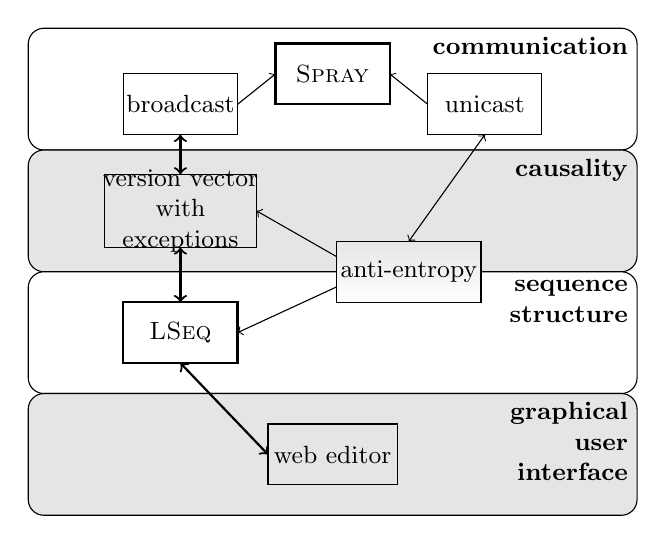
\begin{tikzpicture}[scale=1.1]

\newcommand\X{25pt}
\newcommand\Y{20pt}

\newcommand\LIGHTGRAY{gray!20}

\small
%% communication
\draw[rounded corners=2mm, fill=white](0pt, 0pt)+(-4*\X,-\Y)rectangle+(4*\X,\Y);
\draw(4*\X, \Y)node[anchor=north east]{\textbf{communication}};

\draw[fill=white](-2*\X, -0.25*\Y)
node{broadcast}+(-0.75*\X,-0.5*\Y)rectangle+(0.75*\X,0.5*\Y);
\draw[fill=white, thick]( 0*\X, 0.25*\Y)
node{\SPRAY}+(-0.75*\X,-0.5*\Y)rectangle+(0.75*\X,0.5*\Y);
\draw[fill=white]( 2*\X, -0.25*\Y)
node{unicast}+(-0.75*\X,-0.5*\Y)rectangle+(0.75*\X,0.5*\Y);

\draw[<-](-0.75*\X, 0.25*\Y)--(-1.25*\X, -0.25*\Y);
\draw[<-](0.75*\X, 0.25*\Y)--(1.25*\X, -0.25*\Y);

%% causality
\draw[rounded corners=2mm, fill=\LIGHTGRAY](0pt, -2*\Y)+(-4*\X,-\Y)rectangle+(4*\X,\Y);
\draw(4*\X, -\Y)node[anchor=north east]{\textbf{causality}};

\draw[fill=\LIGHTGRAY](-2*\X, -2*\Y)
node[align=center]{version vector\\with\\exceptions}
+(-1.0*\X,-0.6*\Y)rectangle+(1.0*\X,0.6*\Y);

\draw[<->, thick](-2*\X, -0.75*\Y)--(-2*\X, -1.4*\Y);
\draw[<->]( 2*\X, -0.75*\Y)--( 1*\X, -2.5*\Y);

%% sequence structure
\draw[rounded corners=2mm, fill=white](0pt, -4*\Y)+(-4*\X,-\Y)rectangle+(4*\X,\Y);
\draw(4*\X, -3*\Y)node[anchor=north east, align=right]
{\textbf{sequence}\\\textbf{structure}};

\draw[fill=white, shading=axis,top color=\LIGHTGRAY, bottom color=white, shading angle=0](1*\X, -3*\Y)
node{anti-entropy}+(-0.95*\X,-0.5*\Y) rectangle +(0.95 *\X, 0.5*\Y);
\draw[fill=white, thick](-2*\X, -4*\Y)
node{\LSEQ}+(-0.75*\X,-0.5*\Y) rectangle +(0.75 *\X, 0.5*\Y);

\draw[->] (0.05*\X, -2.75*\Y)--(-1*\X,-2*\Y);
\draw[->] (0.05*\X, -3.25*\Y)--(-1.25*\X,-4*\Y);
\draw[<->, thick] (-2*\X, -3.5*\Y)--(-2*\X, -2.6*\Y);

%% gui
\draw[rounded corners=2mm, fill=\LIGHTGRAY](0pt, -6*\Y)+(-4*\X,-\Y)rectangle+(4*\X,\Y);
\draw(4*\X, -5*\Y)node[anchor=north east, align=right]
{\textbf{graphical}\\\textbf{user}\\\textbf{interface}};
\draw[fill=\LIGHTGRAY](0pt,-6*\Y)
node{web editor}+(-0.85*\X,-0.5*\Y) rectangle +(0.85 *\X, 0.5*\Y);

%%\draw[<->] (-2*\X, -4.5*\Y) -- (0*\X, -5.5*\Y);
\draw[<->, thick] (-2*\X, -4.5*\Y) -- (-0.85*\X, -6*\Y);
\end{tikzpicture}
  \caption{\label{fig:architecture}The four layers of \CRATE's architecture}
\end{figure}

\subsection{Communication}
To collaboratively edit a document, users must establish a form of communication
between them. It firstly requires to build a network of communication
channels. It secondly requires to use it to disseminate the changes performed on
the shared document to all participants.  \CRATE uses
\SPRAY~\cite{nedelec2015spray} as membership protocol and relies on its
properties to efficiently disseminate the messages.

\begin{asparadesc}
\item [The membership protocol,] called \SPRAY, is a random peer sampling
  protocol~\cite{jelasity2007gossip} the primary target of which is WebRTC, a
  recent technology that allows peer-to-peer communication between web browsers.
  As such, the range of users includes small devices (e.g. smartphones, tablets,
  etc.) and establishing a connection requires a three-way handshake. These
  constraints invite to maintain a small number of connections.

  Using \SPRAY, each member owns a set of neighbors which dynamically grows and
  shrinks to reflect the network size. Without any global knowledge,
  \begin{inparaenum}[(i)]
  \item it provides each member with a neighborhood of logarithmic size compared
    to the global network size;
  \item it quickly converges to a topology exposing similarities with random
    graphs~\cite{erdos1959random}. Among others,
    \begin{inparaenum}[(a)]
    \item it balances the load among members by repeatedly averaging over time the
      size of neighborhoods pairwise;
    \item it becomes robust to random crashes or unexpected departures of
      members;
    \item the shortest average distance to reach all peers stays small.
    \end{inparaenum}
  \end{inparaenum}
  
  \SPRAY divides the life-cycle of a member into three phases: the joining, the
  exchanges, and the leaving. They respectively aim to increase, retain, and
  decrease the number of connections to follow a logarithmic progression.

\item [The information dissemination protocol]\cite{birman1999bimodal} aims to
  propagate the changes performed by the user on their shared document. Any
  operation must reach all members (broadcast) to guarantee eventual
  consistency. The dissemination relies on the neighborhood provided by
  \SPRAY. When a user performs an operation, \CRATE prepares a message including
  the result of the operation and sends it to the whole network using its
  neighborhood. Neighbors receiving such message forward it to their own
  neighbors. Hence, messages reach all participants transitively. To guarantee
  termination and limit the flooding, each member forwards each message to their
  neigbhors only once by using a version vector with exceptions
  (cf. Section~\ref{subsec:causality}).

  The information dissemination protocol impacts the communication complexity at
  each peer:
  \begin{equation}
    \mathcal{O}(m.\ln |\mathcal{R}| )
  \end{equation}
  where $m$ is the message size determined by the layers below, and
  $|\mathcal{R}|$ is the number of replicas in the network including both
  writers and readers of the shared sequence.
\end{asparadesc}

\subsection{Causality tracking}
\label{subsec:causality}

The causality tracking layer guarantees that operations are not delivered more
than once, and that operations depending on another operation is delivered after
the latter. \CRATE uses a version vector with
exceptions~\cite{malkhi2007concise} which stores for each site
\begin{inparaenum}[(i)]
\item an integer denoting the maximum counter of operations originated from this
  site and
\item a list of integers denoting the exceptions, i.e., the counter of
  operations known as not received yet.
\end{inparaenum}

Each operations is uniquely identified by its unique site identifier and a
monotonically growing counter. On operation reception, \CRATE discards the
operation if it has already been received before. Otherwise, it modifies the
version vector entry either by updating the maximum counter or removing an entry
in the exceptions.

\begin{figure}
  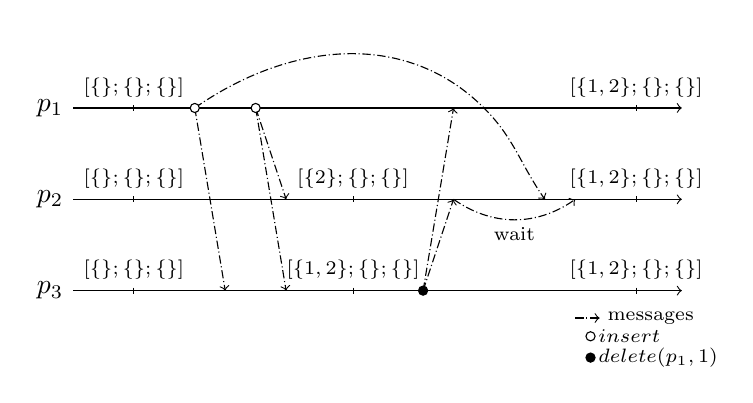
\begin{tikzpicture}[scale=1.1]
  
  \draw (-10pt,0pt) node[anchor=east]{$p_1$};
  \draw (-10pt,-30pt) node[anchor=east]{$p_2$};
  \draw (-10pt,-60pt) node[anchor=east]{$p_3$};

  \draw[->] (-10pt,0pt) -- (190pt,0pt);
  \draw[->] (-10pt,-30pt) -- (190pt,-30pt);
  \draw[->] (-10pt,-60pt) -- (190pt,-60pt);

  \scriptsize
  \draw (10pt,1pt) node[anchor=south]{[$\{\};\{\};\{\}]$} --
  (10pt,-1pt);
  \draw (10pt,-29pt) node[anchor=south]{[$\{\};\{\};\{\}]$} --
  (10pt,-31pt);
  \draw (10pt,-59pt) node[anchor=south]{[$\{\};\{\};\{\}]$} --
  (10pt,-61pt);

  \draw[->,densely dashdotted] (30pt,0pt) -- (40pt,-60pt);
  \draw[->,densely dashdotted] (50pt,0pt) -- (60pt,-30pt);
  \draw[->,densely dashdotted] (50pt,0pt) -- (60pt,-60pt);


  \draw (82pt,-29pt) node[anchor=south]{[$\{2\};\{\};\{\}]$} --
  (82pt,-31pt);
  \draw (82pt,-59pt) node[anchor=south]{[$\{1,2\};\{\};\{\}]$} --
  (82pt,-61pt);

  \draw [->,densely dashdotted] (30pt,0pt) to[out=35,in=135] (125pt,0pt)
  to[out=-45,in=125] (145pt,-30pt);

  \draw[fill=white] (30pt,0pt) circle (1.5pt);
  \draw[fill=white] (50pt,0pt) circle (1.5pt);

  \draw[->,densely dashdotted] (105pt,-60pt)--(115pt,-30pt);
  \draw[->,densely dashdotted] (105pt,-60pt)--(115pt,0pt);

  \draw[fill=black] (105pt,-60pt) circle (1.5pt);
  
  \draw[->,densely dashdotted]
  (115pt,-30pt)to[out=-35,in=-145]node[anchor=north]{wait}(155pt,-30pt);


  \draw (175pt,1pt) node[anchor=south]{$[\{1,2\};\{\};\{\}]$}-- (175pt,-1pt);
  \draw (175pt,-29pt) node[anchor=south]{$[\{1,2\};\{\};\{\}]$}--(175pt,-31pt);
  \draw (175pt,-59pt) node[anchor=south]{$[\{1,2\};\{\};\{\}]$}--(175pt,-61pt);
  
  \draw[->,densely dashdotted] (155pt,-69pt) -- (163pt,-69pt)
  node[anchor=west]{messages};
  \draw[fill=white] (160pt,-75pt)node[anchor=west]{$insert$}circle (1.5pt);
  \draw[fill=black] (160pt,-82pt)
  node[anchor=west]{$delete(p_1,1)$} circle (1.5pt);

\end{tikzpicture}

  \caption{\label{fig:timeline}Causality tracking example.}
\end{figure}

Figure~\ref{fig:timeline} depicts a scenario where 3 peers are involved. Thus,
all peers have a vector of three entries. Peer $p_1$ inserts two elements in the
sequence and broadcasts the operations. Peer $p_3$ immediately receives both
operations and increments the entry in its version vector accordingly.  In the
meantime, Peer $p_2$ only receives the second operation which leads to an update
of the maximum counter and an exception concerning the first operation of Peer
$p_1$. Then, Peer $p_3$ removes the first element inserted by $p_1$ and
broadcast it. While $p_1$ delivers the removal immediately, Peer $p_2$ has to
wait since the targeted operation belongs to the exceptions. Once it receives
the first operation of $p_1$, the exception disappears and the delete operation
is performed.

The local space complexity of such data structure depends of the number of
writers $|\mathcal{W}|$, i.e., the users that modified the document at least
once:
\begin{equation}
  \mathcal{O}(|\mathcal{W}|)
\end{equation}
The communication complexity is not impacted from this data
structure. Therefore, its becomes:
\begin{equation}
  \mathcal{O}(o.\ln |\mathcal{R}|)
\end{equation}
where $o$ is the operation size determined by the shared sequence structure,
and the rest is determined by the communication layer.

The anti-entropy periodically checks if the local replica diverges from another
neighbor's one at random. It aims to retrieve missing operations that could have
been lost during the transmissions. \TODO{example}. There is no additional cost
on local memory. However, the communication cost is prohibitively high which
encourages to perform this reconciliation protocol with great care:
\begin{equation}
  \mathcal{O}(|\mathcal{W}|+|\mathcal{W}|+x.o)
\end{equation}
where the first $|\mathcal{W}|$ designates the initiating message, and
$|\mathcal{W}|+x.o$ the response to this message where $x.o$ are the missing
operations.

\subsection{Shared sequence}
The shared sequence layer uses a conflict-free replicated data type for
sequences~\cite{shapiro2011comprehensive, shapiro2011conflict}. It is an
abstract data type for sequences that provides two commutative operations:
insert and delete. As such, the delivery order of operations does not matter as
long as the deletion of an element follows its insertion. This property makes
these shared sequences tolerant to concurrency. However, their complexity lies
in their space consumption. Indeed, each insert operation allocates a unique and
immutable identifier to the element. A global total order among the identifiers
guarantees that replicas eventually converge to an identical states.

\CRATE uses \LSEQ, a polyLogarithmic identifier allocator for SEQuences. Its
underlying structure is an exponential tree which, when linearized using its
global total order, results in the sequence of elements representing the
document. \LSEQ comprises two parts:
\begin{inparaenum}[(i)]
\item the function $allocPath$ which chooses the path in the tree for the
  newly allocated identifier.
\item the function $allocDis$ which decorates the path in order to ensure its
  uniqueness even in presence of concurrent insertions.
\end{inparaenum}

The function $allocPath$ chooses the path associated with each element in order
to encode its relative position with regard to its adjacent elements in the
sequence. For the sake of performance, the aim of $allocPath$ is to keep the
underlying tree with a small depth. Three components compose $allocPath$. Each
of these components fails to provide an efficient allocation
function. Nevertheless, their composition allows to get the best of each by
canceling their respective deficiency.
\begin{asparadesc}
\item [An exponential tree]~\cite{andersson1996faster,andersson2007dynamic}
  represents the shared document. The path is a sequence of numbers chosen among
  a subset of numbers the size of which is doubled at each concatenation. For
  instance, if a path $p_1$ of size 1 is chosen among [$\mathbb{N}_{<32}$], a
  path $p_2$ of size 2 is chosen among [$\mathbb{N}_{<32}.\mathbb{N}_{<64}$]
  etc. Let $r$ be the number of possible paths with one concatenation (i.e., the
  maximum arity of the root of the tree), a path $p_k$ of size $k$ is chosen
  among [$\mathbb{N}_{<r}.\mathbb{N}_{<2r}\ldots\mathbb{N}_{<2^{k-1}r}$].  Due
  to the growth of the subsets, such representation of the paths requires one
  additional bit to encode each concatenation. With the same examples, it
  implies that $p_1$ is encoded using $log_2(32)=5$ bits, $p_2$ is encoded using
  $5+6=11$ bits,~\ldots Thus, a path is encoded by:
  \begin{equation}
    \sum\limits_{i=1}^{k}(\log_2(r)+i) =
    k\log_2(r) + {k(k+1)\over{2}} = \mathcal{O}(k^2) \,\, bits
  \end{equation}
  When an exponential tree of depth $k$ is balanced (i.e., all its branches
  are filled) it holds uptil:
  \begin{equation} \sum\limits_{i=0}^{k-1} {2^{(i^2-i)/2}} \,\, elements
  \end{equation}
  When an exponential tree of depth $k$ has one branch filled per level, it
  holds uptil:
  \begin{equation} 2^{k+1}-1 \,\, elements\end{equation} 
  In the worst case, the tree contains one element per level.
  
  An alphabetical order maintains a dense total order among elements in the
  tree. It primary uses the path of elements alongside globally unique markers
  called disambiguators. The latter's objective is twofold:
  \begin{inparaenum}[(i)]
  \item to order concurrent operations that happen to have an identical path and
  \item to allow the allocation of new identifiers in-between them.
  \end{inparaenum}
  For instance, let [3] be the path of Element Q inserted by User $u_x$, and let
  [4] the path of Element T inserted by User $u_y$. When a user $u_1$ inserts W
  between those elements, the depth of the tree must grow to welcome the new
  element. Assuming that depth 1 has a maximum arity of 8, the identifier is
  allocated in the range from [3.0] to [3.15].  In this example, the resulting
  path is [3.6]. In the meantime, another user $u_2$ inserts R between Q and T
  which happens to result in the path [3.6] too. To ensure a total order,
  disambiguators are associated with each path composed of a monotonically
  growing counter and a globally unique site identifier. Here, the identifier of
  Element W is composed of the path [3.6] and disambiguator
  [$\langle u_x,\,1\rangle$, $\langle u_1,\,1$] and the Element R is composed of
  the path [3.6] and disambiguator [$\langle u_x,\,1\rangle$,
  $\langle u_2,\,1\rangle$].  The comparison starts to examine the first
  concatenations which are equal.  Then, the comparison concerns the path of the
  second level of the tree which are equals too. Hence, it examines the
  disambiguators to determine that W is located before R because $u_x < u_y$ in
  this case. The resulting sequence is QWRT.
  
\item [Two sub-allocation functions] designed for monotonic editing, i.e.,
  inserting repeatedly at an adjacent position of the previously inserted
  element. These are application dependent. While one is well-suited to
  end-editing (left-to-right), the other is well-suited for front-editing
  (right-to-left). To achieve this, they respectively allocate paths close of
  the leftmost path, and rightmost path in order to preserve space for the
  future insertions. Hence, the left-to-right allocation function leaves
  available paths at the right of the tree, while the right-to-left function
  aims the opposite. For instance, a user writes QWERTY starting from the Q to
  the Y. Using the left-to-right allocation function leads to identifiers like
  [2], [4], [7], [7.2], [7.5], [7.9]. Small space is left in-between paths to
  handle mistakes, e.g., a user misses some characters while typing.  Since
  accurately predicting the editing behavior of users is \TODO{impossible},
  \LSEQ uses these two antagonist strategies to adapt to any editing behaviors
  assuming that edition is mostly about compositions of sequences of monotonic
  insertions.
  
\item [A hash function] chooses among the two sub-allocation functions. The
  choice is made randomly using a hash function following a uniform
  distribution. Such function does not favor any editing behavior while
  remaining efficient. This provides the independence of the allocation function
  from any editing strategy. Furthermore, as shown
  in~\cite{nedelec2013concurrency}, using antagonist sub-allocation functions
  forces all peers to make identical choices. To reach that goal, they all use a
  similar hash function initialized with a common seed and shared within the
  document. When a user inserts a new element in the sequence, \LSEQ firstly
  processes the depth of the new path, and secondly defers the allocation to the
  function designated by the hash of the depth.
\end{asparadesc}

% \begin{algorithm}[h]
%   
\begin{algorithmic}[1]

\small
\algrenewcommand{\algorithmiccomment}[1]{\hskip2em$\rhd$ #1}
\newcommand*{\comment}[1]{$\rhd$ #1}

  \State \textbf{let} $boundary \leftarrow 10$; \hfill \comment{Any constant}
  \label{line:boundary}
  \State \textbf{let} $h:\mathbb{N} \rightarrow (\mathcal{P}\times
  \mathcal{P}\rightarrow \mathcal{P})$; \hfill \comment{get sub-allocation
    function}
  \Statex
    \Function{allocPath}{$p,\, q \in \mathcal{P}$}
    $\rightarrow \mathcal{P}$
    \State \textbf{let} $\langle depth,\,\_ \rangle 
    \leftarrow \textsc{getDepthInterval}(p,\,q)$;
    \State \textbf{return} $h(depth)(p,\,q)$; 
    \hfill \comment{Delegates the call}
    \EndFunction
    \Statex
    \Function{left-to-right}{$p,\,q \in \mathcal{P}$}\label{line:lefttoright}
    $\rightarrow \mathcal{P}$
    \Statex \comment{\#1 Get the depth of the new path}
    \State \textbf{let} 
    $\langle depth,\,interval \rangle \leftarrow \textsc{getDepthInterval}(p,\,q);$
    \Statex \comment{\#2 Maximal space between two identifiers}
    \State \textbf{let} $step \leftarrow min(boundary,\,interval)$;
    \Statex \comment{\#3 Create the new path}\label{line:plus}
    \State \textbf{return} $\textsc{subPath}(p,\,depth) + rand(0,\,step)$;
    \EndFunction
    \Statex
    \Function{right-to-left}{$p,\,q \in \mathcal{P}$}\label{line:righttoleft}
    $\rightarrow \mathcal{P}$
    \State \textbf{let}
    $\langle depth,\, interval\rangle \leftarrow \textsc{getDepthInterval}(p,\,q);$
    \hfill \comment{\#1}
    \State \textbf{let} $step \leftarrow min(boundary,\,interval)$;
    \hfill \comment{\#2}
    \State \textbf{return} $\textsc{subPath}(q,\,depth) - rand(0,\,step)$;
    \hfill \comment{\#3}\label{line:minus}
    \EndFunction
    \Statex
    \Function{getDepthInterval}{$p,\,q \in \mathcal{P}$} $\rightarrow \mathbb{N} \times \mathbb{N}$
    \Statex   \comment{Which level has enough space for 1 path} 
      \State \textbf{let} $d \leftarrow 0$; \hfill \comment{depth}
      \State \textbf{let} $interval \leftarrow 0$;
      \While{$(interval < 2)$}
        \State $d \leftarrow d + 1$;
        \State $interval \leftarrow \textsc{subPath}(q,\,d) - \textsc{subPath}(p,\,d)$;
      \EndWhile
      \State \textbf{return} $\langle d,\, interval\rangle$;
    \EndFunction

  \end{algorithmic}


%   \caption{The $allocPath$ function of \LSEQ}
%   \label{algo:allocpathalgo}
% \end{algorithm}
  

% \begin{algorithm}
%   \input{input/allocdesalgo.tex}
%   \caption{\label{algo:allocdis}The function $allocDis$ of \LSEQ}
% \end{algorithm}

% In text editing, most of the editing behaviors can be empirically summarized
% as a composition of two basic editing behaviors.
% \begin{inparaenum}[(i)]
% \item The random editing behavior where the author inserts new elements at
%   what appears random positions in the sequence. For instance, this behavior
%   mostly arises when syntactic corrections are performed, e.g., the author
%   writes $QWETY$ and realizes that the $R$ is missing. She adds the missing
%   character in a second time.
% \item The monotonic editing behavior where the author repeatedly inserts new
%   elements between the last inserted element and an adjacent element (after or
%   before exclusively). For instance, when an author writes $QWERTY$, she
%   generally starts from the first letter $Q$ to the last letter of the word
%   $Y$. On the opposite, insertions in a logfile are usually performed at the
%   beginning for practical reasons.
% \end{inparaenum}

% As a consequence, we focus on the space complexity analysis of \LSEQ to
% random and monotonic editing behaviors to which we add a worst-case complexity
% analysis.  The analysis does not include an average case since it requires to
% know the average distribution of the position of edits performed by a human
% collaborator which is obviously very complex.

\begin{table*}
  \centering
  
\begin{tabular}{@{}lccccccc@{}}
  \toprule
  \textsc{Editing behavior} & \multicolumn{2}{c}{\textsc{Space}} & \multicolumn{5}{c}{\textsc{Time}} \\ \cmidrule{4-8}
  & & & \multirow{2}{*}{\textsc{Lookup}} & \multicolumn{2}{c}{\textsc{Local}} & \multicolumn{2}{c}{\textsc{Remote}} \\ \cmidrule{2-3} \cmidrule{5-8}
  & \textsc{Identifier} & \textsc{Sequence} & & \textsc{ins} & \textsc{del} & \textsc{ins} & \textsc{del}  \\ \midrule
  Random editing & $\mathcal{O}(\log I)$ & $\mathcal{O}(I\log I)$ & $\mathcal{O}(2^{\sqrt{\log I}})$ & $\mathcal{O}(\sqrt{\log I})$ & $\mathcal{O}(1)$ & $\mathcal{O}(\log I + \sqrt{\log I})$ & $\mathcal{O}(\log I + \sqrt{\log I})$ \\
  Monotonic editing & $\mathcal{O}((\log I)^2)$ & $\mathcal{O}(I \log I)$ & $\mathcal{O}(I)$ & $\mathcal{O}(\log I)$ & $\mathcal{O}(1)$ & $\mathcal{O}((\log I)^2 +\log I)$ & $\mathcal{O}((\log I)^2 +\log I)$ \\
  Worst case & $\mathcal{O}(I^2)$ & $\mathcal{O}(I^2)$ & $\mathcal{O}(I)$ & $\mathcal{O}(I)$ & $\mathcal{O}(1)$ & $\mathcal{O}(I)$ & $\mathcal{O}(I)$\\ \bottomrule
\end{tabular}


%%  Id.size & $O(\sqrt{log\,n})$ & $O(log\,n)$ & $O(n)$ \\ \midrule
%%  Id.bit-length & \multicolumn{3}{c}{ $\sum\limits_{i=1}^{k}b+i =
%%                  kb + k(k+1)/2 = O(k^2)$} \\ \midrule
%%  Space complexity & $O(log\,n)$ & $O((log\,n)^2)$ & $O(n^2)$ \\ \bottomrule
  \caption{\label{table:lseqcomplexities}
    Upper-bound on space and time complexities of \LSEQ. Where $I$ is the number
    of insert operations performed.}
\end{table*}

\TODO{To summarizes, the space complexity analysis reveals that the allocation
function \LSEQ sacrifices on the worst-case space complexity to improve the
space complexity of the monotonic editing behaviors. Nevertheless, in text
editing, the worst-case happens with a very low probability compared the other
cases. Furthermore, it is worth noting that usually, the authors do not write a
document in a single round, starting from the beginning to go straight up to
the end (as the monotonic analysis could suggest). On the contrary, the authors
write sections, structure the documents, perform corrections, rewrite parts of
the document, reorganize, etc. This behavior (between random and monotonic
behavior) tends to even up the branches of the underlying tree of \LSEQ. In
the case of random editing, the space complexity is asymptotically optimal
$O(log\,n)$ while it is very interesting in a "normal setting" $O((log\,n)^2)$.}

\begin{figure*}
  \centering
  \subfloat {\input{input/lseqtreeexampleA.tex}}
  \hspace{10pt}
  \subfloat {\input{input/lseqtreeexampleB.tex}}
  \caption{\label{fig:lseqtreeexample}\LSEQ tree handling two monotonic
    editing behaviors.}
\end{figure*}


Figure~\ref{fig:lseqtreeexample} depicts the resulting trees after two
antagonist scenarios creating the sequence $QWERTY$
\begin{inparaenum}[(i)] 
\item the left-to-right editing sequence [($Q,\,0$), ($W,\,1$), \ldots] and
\item the right-to-left editing sequence [($Y,\,0$), ($T,\,0$), \ldots].
\end{inparaenum}
In both cases, the exponential tree of \LSEQ starts with an arity $32$ and
doubles it at each level. Also, it uses the $frontEditing$ and $endEditing$
sub-allocation functions at the first and the second level of the tree
respectively. Since the first level of the tree uses the function $endEditing$,
the scenario involving the left-to-right editing sequence results in a tree of
depth 1. On the other hand, contrarily to the allocation function presented in
Figure\ref{fig:allocpathexample}), the antagonist scenario does not increase
very much the depth of the tree. Indeed, the identifiers of \LSEQ quickly reach
a level of the tree where the sub-allocation function is designed to handle the
right-to-left editing behavior.


%%% Local Variables: 
%%% mode: latex
%%% TeX-master: "../paper"
%%% End: 

% LocalWords:  disambiguator neighbours

\section{Experiments}
\label{sec:experiments}

This section is divided into two parts. The first part describes the core of
the distributed CollaboRATive Editor \CRATE by filling in the blanks
left on causality tracking and eventual delivery of operations. The second part
concerns the experiments that aim to:

\begin{enumerate}[leftmargin=*]
\item Validate the space complexity of \LSEQ and highlight the improvement
  over the state-of-the-art.
\item Show that \CRATE scales with respect to the number of
  collaborators simultaneously involved in a document editing.
\item Show that concurrency does not impact the size of
  identifiers. Consequently, the space complexity of the identifiers can be
  studies in scenarios without concurrency.
\end{enumerate}

\subsection{CRATE}
\label{subsec:crdt}
\CRATE (CollaboRATive Editor) is a prototype of decentralised editor. We
assume that collaborators can join the document editing and leave when they
want. The group of collaborators can be seen as a peer-to-per network. Hence,
\CRATE uses a gossip dissemination protocol to scale with respect to the
number of collaborators/peers involved in the authoring. In this protocol, each
peer has a set of neighbours and communicates with them. When a peer performs
an operation, it creates a message containing the result of the operation. Each
peer broadcasts its messages and when a peer receives a specific message for
the first time, it re-broadcasts this message. However,
Section~\ref{sec:preliminaries} states that strong eventual consistency is
ensured upon the assumption of eventual delivery, and unfortunately, the
gossiping broadcast is only reliable with high probability. To make it
reliable, \CRATE includes an additional anti-entropy protocol to
retrieve the possibly missing operations (cf.~\ref{sec:messagedelivery}).

Section~\ref{sec:preliminaries} also states that sequences can be seen as
conflict-free data types under the condition that deletion of a particular
element cannot precede its insertion. To ensure this condition, \CRATE
uses a vector structure called interval version
vector~\cite{mukund2014optimized} (IVV) whose values are version numbers called
dates.

Similarly to version vectors, IVVs require a vector with one entry per peer
involved in the authoring at the difference that each entry of an IVV contains
a vector of intervals. Furthermore, when a peer broadcasts an operation, only
two scalars are required to preserve the causal dependency instead of a full
vector. This difference considerably lowers the network overload while keeping
a local space complexity of the same order than version vectors.  It
constitutes an essential trade-off since local memory is often considered as
virtually infinite while the network can be easily overloaded. \CRATE
uses an IVV to
\begin{inparaenum}[(i)]
\item minimise the retransmission of operations (i.e. each peer broadcast only
  once each operation),
\item integrate the insert operation only once,
\item preserve the aforementioned invariant.
\end{inparaenum}
The delivery algorithm using the IVV can be found in~\ref{sec:messagedelivery}.

\begin{figure}
  \centering 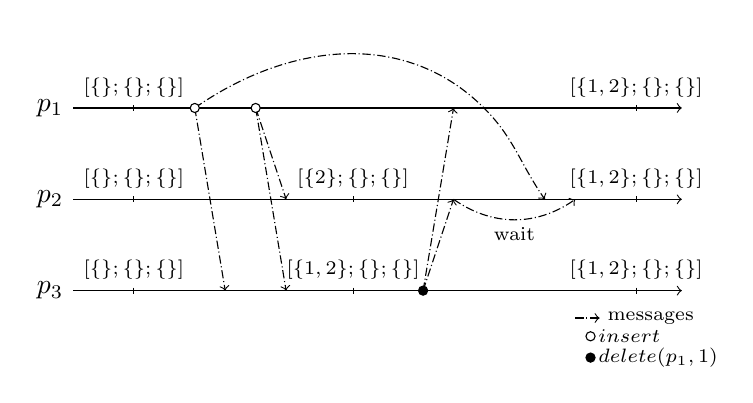
\begin{tikzpicture}[scale=1.1]
  
  \draw (-10pt,0pt) node[anchor=east]{$p_1$};
  \draw (-10pt,-30pt) node[anchor=east]{$p_2$};
  \draw (-10pt,-60pt) node[anchor=east]{$p_3$};

  \draw[->] (-10pt,0pt) -- (190pt,0pt);
  \draw[->] (-10pt,-30pt) -- (190pt,-30pt);
  \draw[->] (-10pt,-60pt) -- (190pt,-60pt);

  \scriptsize
  \draw (10pt,1pt) node[anchor=south]{[$\{\};\{\};\{\}]$} --
  (10pt,-1pt);
  \draw (10pt,-29pt) node[anchor=south]{[$\{\};\{\};\{\}]$} --
  (10pt,-31pt);
  \draw (10pt,-59pt) node[anchor=south]{[$\{\};\{\};\{\}]$} --
  (10pt,-61pt);

  \draw[->,densely dashdotted] (30pt,0pt) -- (40pt,-60pt);
  \draw[->,densely dashdotted] (50pt,0pt) -- (60pt,-30pt);
  \draw[->,densely dashdotted] (50pt,0pt) -- (60pt,-60pt);


  \draw (82pt,-29pt) node[anchor=south]{[$\{2\};\{\};\{\}]$} --
  (82pt,-31pt);
  \draw (82pt,-59pt) node[anchor=south]{[$\{1,2\};\{\};\{\}]$} --
  (82pt,-61pt);

  \draw [->,densely dashdotted] (30pt,0pt) to[out=35,in=135] (125pt,0pt)
  to[out=-45,in=125] (145pt,-30pt);

  \draw[fill=white] (30pt,0pt) circle (1.5pt);
  \draw[fill=white] (50pt,0pt) circle (1.5pt);

  \draw[->,densely dashdotted] (105pt,-60pt)--(115pt,-30pt);
  \draw[->,densely dashdotted] (105pt,-60pt)--(115pt,0pt);

  \draw[fill=black] (105pt,-60pt) circle (1.5pt);
  
  \draw[->,densely dashdotted]
  (115pt,-30pt)to[out=-35,in=-145]node[anchor=north]{wait}(155pt,-30pt);


  \draw (175pt,1pt) node[anchor=south]{$[\{1,2\};\{\};\{\}]$}-- (175pt,-1pt);
  \draw (175pt,-29pt) node[anchor=south]{$[\{1,2\};\{\};\{\}]$}--(175pt,-31pt);
  \draw (175pt,-59pt) node[anchor=south]{$[\{1,2\};\{\};\{\}]$}--(175pt,-61pt);
  
  \draw[->,densely dashdotted] (155pt,-69pt) -- (163pt,-69pt)
  node[anchor=west]{messages};
  \draw[fill=white] (160pt,-75pt)node[anchor=west]{$insert$}circle (1.5pt);
  \draw[fill=black] (160pt,-82pt)
  node[anchor=west]{$delete(p_1,1)$} circle (1.5pt);

\end{tikzpicture}

  \caption{\label{fig:timelineexample}Timeline of operations performed by 3
    collaborators. For the sake of simplicity, sets represent the intervals
    stored in the local vectors. In this example, the $insert$ operations
    concern any element while the $delete$ operation targets the first
    insertion of collaborator $p_1$.}
\end{figure}

Figure~\ref{fig:timelineexample} depicts an example of causality tracking using
an IVV with all possible configurations. Each of the three peers initialises
its 3-entry vector with empty intervals. First, peer $p_1$ performs an
insertion and broadcasts it to $p_2$ and $p_3$. The operation conveys the
unique peer identifier $p_1$ and its corresponding stamp $1$. When $p_3$
receives the message, it adds the entry to the corresponding interval, and
immediately delivers the new element. The second operation of $p_1$ conveys the
stamp $2$. When $p_2$ receives this message, it merges the entry with its local
vector and delivers the element, even if the first operation of $p_1$ is not
received yet. Peer $p_3$ does the same resulting in the intervals
$[\{1,2\};\{\};\{\}]$. Then, $p_3$, not satisfied by the first operation of
$p_1$ deletes it. The message conveys these two scalars. When $p_2$ receives
the message, the interval corresponding to the insertions at $p_2$ does not
contain the first one. Consequently, the $del$ operation must wait the delivery
of the first insertion of $p_1$. On $p_1$, the $del$ operation is immediately
delivered.

\subsection{Setup and results}

Two kinds of environments hosted the experiments. First, a single machine
emulating multiple peers. Despite the poor scalability of these experiments due
to replication, it allows running the experiments in a controlled
environment. Then, multiple machines distributed in a cluster of the Grid'5000
testbed are considered. A single machine can host multiple peers and
communicate with other machines. The magnitude of these experiments grows up to
$450$ connected peers.

In these experiments, we focus our analysis on two editing behaviours: random
and monotonic. In random editing, when a peer inserts an element, it randomises
the position of the new element in the document following a uniform
distribution. In monotonic editing, when a peer inserts an element, it inserts
the new element at the end of the document. As stated in
Section~\ref{sec:spacecomplexity}, this case is not favourable because it tends
to unbalance the underlying tree representing the sequence. In contrast to
this, performing insertions at different locations tends to even up the branch
of the tree, i.e., the average size of identifiers is lowered.

We focus our measurements on the average size of the messages broadcast by each
peer. Since the delete messages have a low and constant size, we focus on
messages corresponding to insert operations. Therefore, the measurements
reflect the average size of the identifiers. The initial base parameter, i.e.,
the maximum number of children at the root of the exponential tree, starts from
a low value in order to accelerate the growth of the identifiers. In this
section, we are more interested in the shape of the curves than in the actual
values.

In order to perform these evaluations, we developed a JavaScript data type for
Web applications. The code is released on the Github
platform\footnote{\url{https://github.com/Chat-Wane/LSEQTree.git}} under the
MIT license. Based on this implementation, we developed a prototype of
distributed CollaboRATive Editor
\CRATE\footnote{\url{https://github.com/Chat-Wane/CRATE.git}} following
the outlines of this paper.
\ \\

\begin{asparadesc}
\item [Objective:] Validate the space complexity analysis of \LSEQ. In
  particular, when the editing behaviour is monotonic, \LSEQ has a
  polylogarithmic upper-bound on space complexity with respect to the number of
  insert operations. When the editing behaviour is random, \LSEQ has a
  logarithmic space complexity. A second objective is to compare \LSEQ with
  an existing sequence structure
  Logoot~\cite{weiss2009logoot,weiss2010logootundo}.
\item [Description:] A single machine hosts two peers communicating via a
  peer-to-peer connection. They produce a document of half a million characters
  in $50$ minutes, i.e., they insert $166$ characters per second. Two editing
  behaviours are studied: monotonic and random. They use either \CRATE,
  or a version of \CRATE using Logoot instead of \LSEQ. According
  to~\cite{ahmed2011evaluating}, Logoot constitutes the sequence with
  variable-size identifiers that delivers the best performance overall. As
  such, it is an ideal baseline. While \LSEQ starts with a departure base of
  $2^8$ and doubles it when required, Logoot uses a constant base of
  $2^{16}$. We measure the average size of messages transiting through the
  peers during the experiment.

\begin{figure}
  \centering
  \includegraphics[angle=-90,width=0.475\textwidth]{./img/complexities.eps}
  \caption{\label{fig:complexities} Average size of the messages exchanged
    between two peers during repeated insertions of elements in the
    sequence. The measurements concern two editing behaviours (monotonic and
    random) with two \CRATE using different sequence structures (Logoot
    and \LSEQ-based). The replicated document grows up to half a million
    characters.}
\end{figure}

\item [Results:] Figure~\ref{fig:complexities} shows the result of the
  experiments. The y-axis corresponds to the average size of messages in
  bytes. The x-axis corresponds to the size of the document, i.e., the number
  of insert operations performed on the sequence. The random editing behaviour
  leads to a logarithmic growth of the size of messages with both sequences
  with a barely noticeable difference. On the other hand, for a monotonic
  editing behaviour Logoot exposes a linear growth of the size of its messages
  while the \LSEQ-based sequence has a polylogarithmic validating the proof
  given in Section~\ref{sec:proposal}. Thus, even if Logoot starts with a
  smaller size messages, it quickly becomes less efficient than the
  \LSEQ-based sequence when the number of insertions increases.

\item [Reasons:] The random editing behaviour is slightly better for the
  \LSEQ-based sequence compared to Logoot because \LSEQ starts with a lower
  departure base. Nonetheless, a random editing behaviour leads to a same space
  complexity for both sequences. For monotonic editing, the identifiers of
  Logoot linearly grow because Logoot uses a K-ary tree. Consequently, it does
  not adapt itself to the growing number of insertions in the sequence, i.e.,
  each node in the tree can store as many nodes as its parent. On the opposite
  side, \LSEQ doubles the number of available children when
  required. Consequently, when the document size increases, the number of
  possible identifiers grows even more.
\end{asparadesc}

\ \\

\begin{asparadesc}
\item [Objective:] Show that \CRATE scales in terms of the number of
  peers. In other words, the size of the network does not impact the space
  complexity upper bound of messages.
\item [Description:] A cluster of the Grid'5000 testbed hosts a varying number
  of peers using the application \CRATE. The peers produce a
  document of 500 thousand characters by repeatedly inserting at the end of the
  document (monotonic editing). The experiments last $50$ minutes. The number
  of peers varies from $2$ to $450$. The generation of $166$ operations
  per second is uniformly distributed among the peers and time. We measure the
  average size of messages.

\begin{figure}
  \centering
  \includegraphics[angle=-90,width=0.475\textwidth]{./img/scalability.eps}
  \caption{\label{fig:scalability}Average size of messages sent during a
    session of document editing. The number of peers varies from $2$ to $450$
    collaboratively producing a document of $500$ thousand characters in $50$
    minutes. The editing behaviour is monotonic.}
\end{figure}

\item [Results:] Figure~\ref{fig:scalability} shows the results of these
  experiments. The y-axis corresponds to the average size of messages in
  bytes. The x-axis corresponds to the number of insert operations performed on
  the sequence. Figure~\ref{fig:scalability} shows that, independently of the
  number of involved peers, the average size of messages grows
  polylogarithmically compared to the size of the document. Also, even if the
  values of the 2-peers curve are invariably above the others, they do not
  demonstrate significant differences. Consequently, \CRATE scales in
  two dimensions: number of peers and number of insertions.
\item [Reasons:] The size of messages reflects the size of the identifiers and
  the additional causality tracking metadata. In Section~\ref{subsec:crdt} that
  describes \CRATE, we saw only two scalars are required to track
  semantically related operations. Since these scalars also exist within the
  identifiers, we reuse them. Consequently, the average size of messages only
  depends of the average size of the identifiers. Since the space complexity of
  \LSEQ is independent of the number of peers, so are the messages of the
  \CRATE. Still, the latter locally requires a linearly growing vector
  in terms of the number of peers. Figure~\ref{fig:scalability} shows small
  measurement variations between the different runs. This result is due to a
  growing number of peers that implies an increasing concurrency rate. When
  some peers perform operations concurrently at a same position, they call the
  function $insert$ with the same bounds as arguments. Therefore the resulting
  paths share a same allocating range. Thus, they are closer from each other
  compared to a sequential execution. Therefore, the average size of messages
  slightly decreases when the number of peers increases.
\end{asparadesc}

\begin{figure}
  \centering
  \includegraphics[angle=-90,width=0.475\textwidth]{./img/latency.eps}
  \caption{\label{fig:latency} Average size of messages sent by peers during
    sessions of document editing. Ten peers produce documents of 10 thousand
    characters by repeatedly inserting at the end of the document at the rate
    of 3 operations per second. Five editing sessions with different network
    latencies are studied.}
\end{figure}

\ \\

\begin{asparadesc}
\item [Objective:] Show that concurrency does not negatively impact the size
  of identifiers. Hence, scenarios without concurrency show the upper-bound on
  the size of identifiers.
\item [Description:] A single machine emulates 10 peers using the application
  \CRATE. The peers produce a document of $10$ thousand characters at a
  rate of 3 insertions per second uniformly distributed among the peers. The
  tool $netem$ provides the network emulation functionality. In particular, it
  allows us to change the transmission delay of messages transmitted through a
  specific network interface. We designed five runs with the approximate
  following latencies: $0.02ms$, $100ms$, $500ms$, $1s$, and $10s$. As usual,
  we measure the average size of the messages.
\item [Results:] Figure~\ref{fig:latency} shows the results of the measurements
  done with the different editing sessions. The y-axis corresponds to the
  average size of messages in bytes and the x-axis corresponds to the number of
  insert operations performed on the sequence. In all cases, the growth of the
  average size of messages follows the expectation given by the space
  complexity analysis in Section~\ref{sec:proposal}. Also, when the latency
  increases, the average size of messages decreases. Thus, the curve that
  corresponds to an almost sequential execution represents the largest
  messages in average.
\item [Reasons:] The explanation behind the decreasing in the average size of
  messages when the latency increases is similar to the one provided in
  previous experiment due to the latency instead of the number of peers.
  Ultimately, when the latency is higher than the run time, each peer of the
  set of collaborator works alone and shares its operations afterwards. The
  resulting tree becomes populated with 10 local executions. Nevertheless, its
  depth does not grow. The bounces in the average message size are due to an
  addition of a level in the paths. Indeed, depending on the depth of the tree,
  the average tends to a specific value. When the depth increases, this average
  value suddenly changes to an higher value. A finer grain of measurements in
  this experiment allows us observing these changes.
\end{asparadesc}

\subsection{Synthesis}
This section detailed a complete distributed collaborative editor.  Using the
outline, we developed \CRATE and used it to perform the experiments. The
first experiment confirmed the space complexity analysis of
Section~\ref{sec:proposal}. Therefore, \CRATE scales with respect to the
number of insert operations performed on the document. The second experiment
showed that using a causality tracking mechanism focused on semantically
dependent operations does not impact the size of messages. As a consequence,
\CRATE scales with respect to the number of peers. Finally, the third
experiment confirmed the observations made in the second one: the concurrency
rate does not negatively impact the size of identifiers. Also, the sequential
execution gives the upper bound on the average size of messages.


%%% Local Variables:
%%% mode: latex
%%% TeX-master: "../paper"
%%% End:



\section{Conclusion}

\label{sec:conclusion}
In the context of collaborative editing, this paper proposed an identifier
allocation function \NAME{} for building sequence replicated data
structures. The obtained sequences enjoy good space and time complexities. The
proof on space complexity demonstrates logarithmic, polylogarithmic, and
quadratic for, respectively, random, monotonic, and worst-case
insertions. Using this allocation function and interval version vectors to
track causality, we developed a distributed collaborative editor called
\EDITORNAME{}. This editor is fully decentralised and scales in terms of the
number of peers, concurrency, and document size. We validated the approach on a
setup close of the real life conditions and using extreme parameters: low
startup values, high number of insertions, high number of peers and high
latency. The experiments confirmed the space complexity of \NAME{} and the
scalability of \EDITORNAME{}. As such, it alleviates the issues brought by
centralised approaches: single point of failure, privacy issues, economic
intelligence issues, limitations in terms of service, etc. Also, it alleviates
the scalability issues of decentralised approaches. As such, it can be seen as
a serious competitor for current trending editors (e.g. Google Docs,
SubEthaEdit,~\ldots), allowing massive collaborative editing without any
service providers. More specifically, it opens the field to a new range of
distributed applications such as massive editing of online courses, or
collaborative reviewing of co-located events, webinars etc.


%% Future work concerns the improvement of our prototype
%% CRATE: \begin{enumerate} \item We aim to develop of a truly tree-based
%% implementation of \NAME{}. Indeed, the current version uses a data structure
%% which is a linearisation of the tree. As a consequence, each element is
%% linked to its identifier without factorising the common parts of the
%% latter. Therefore, the memory usage is currently higher than the one
%% suggested by the theoretical analysis of Section~\ref{sec:proposal}. The
%% network load would remain unchanged.  \item Currently, CRATE only includes
%% the core functionalities described in this paper. However, we intend to add
%% common functionalities such as the modifications of document style, the
%% group awareness, etc.  \item Recent technological advances finally allow to
%% build peer-to-peer applications within the web browser without any
%% additional plug-ins. The real strength of current editors hosted by service
%% providers is their ease of access. Nevertheless, the aforementioned progress
%% puts distributed editors on an equal footing in that regard. Furthermore, it
%% extends the tool to a range of users equipped with small devices but still
%% embedding a web browser such as smartphone users, or Raspberry Pi users
%% etc.  \end{enumerate}

% Future work concerns the causality tracking issue. Indeed, the chosen
% trade-off proposed by the interval version vectors allows scaling in number
% of peers. Nevertheless, when the network is subject to churn, the local
% memory used to store the vector can grow quickly. We envision an approach
% trading accuracy for memory without sacrificing on correctness.

%%% Local Variables: 
%%% mode: latex
%%% TeX-master: "../paper"
%%% End: 

\input{input/acknowledgements.tex}


\bibliographystyle{abbrv}
\raggedright
\bibliography{bibliographie}

% \appendix
% \section{Abstract problem}
\label{sec:problem}
To highlight the problem, we withdraw the unnecessary aspects inherent to CRDTs
and distributed collaborative editing. The ``From Mutable to Immutable'' simply
depicts the problem as a incremental translation from a set where the indices
are mutable, (i.e., an element is linked to a position that may change) to a
set where indices are immutable.
\ \\ \ \\
\textbf{[From Mutable to Immutable problem]} Let $X$ the goal sequence composed
of elements from an alphabet $\mathcal{A}$, $Y$ the sequence resulting of the
permutation of $X$ and containing additional elements from a set $\mathcal{M}$
equipped with a total order $(\mathcal{M},\, <_\mathcal{M})$, $Z$ the set
containing the elements of $X$ and immutable elements from a set $\mathcal{I}$
equipped with a dense total order $(\mathcal{I},\,
<_\mathcal{I})$.\\ \ \\ Given:
\vspace{-\topsep}
\begin{itemize} \itemsep0em
\item $X: \mathbb{N} \rightarrow \mathcal{A}$
\item $Y: \mathbb{N} \rightarrow \mathcal{A} \times \mathcal{M}$
\item $Z: \mathbb{N} \rightarrow \mathcal{A} \times \mathcal{I}$
\item $gen\beta:\mathcal{M} \rightarrow \mathcal{I}$
\item $Z$-uniqueness:\\ $\forall\langle \alpha_1,$ $\beta_1
  \rangle$, $\langle \alpha_2,\beta_2 \rangle \in Z$, $\beta_1
  = \beta_2 \Rightarrow \alpha_1 = \alpha_2$
\item $Z$-order-preservation: $Z(i) = \langle \alpha_i,\, \beta_i\rangle
  \Rightarrow X(i) = \alpha_i$
\item $Z$-specification: ($Z:Y\times\mathbb{N}\rightarrow Z$):
  \vspace{-\topsep}
  \begin{itemize} \itemsep0em
  \item $Z(\varnothing,\,\_\,) \rightarrow \varnothing$
  \item $Z(\_\,,\, 0) \rightarrow \varnothing$
  \item $Z(Y,\, i) \rightarrow$ Let $Y(i) = \langle \alpha_i,\,\mu_i \rangle$:
    $Z(Y,\, i-1) \cup \{\alpha_i,\, gen\beta(\mu_i) \}$
  \item $Z(Y,\,|Y|)$
  \end{itemize}
\end{itemize}
The problem is to find an optimal function $gen\beta$ such that there do not
exist any functions $gen\beta'$ such that for any permutation $Y$, the
resulting set $Z'$ using $gen\beta'$ has a lower binary representation than the
resulting set $Z$ using $gen\beta$.
\ \\

Put back in the distributed collaborative editing context, the goal sequence
$X$ corresponds to the intention of authors, i.e., the final document that
peers will eventually write (e.g., $QWERTY$ in the paper). The sequence $Y$ is
an editing sequence performed by the authors to reach that goal (e.g.,
$[(Q,\,0)$, $(W,\,1)$, $\ldots]$). However, using such indices to order
elements can lead to divergent replicas depending on the integration order. For
instance, let us consider two peers concurrently inserting $(Q,\,0)$ and
$(W,\,0)$. When they receive the operation from each other, the first peer
shifts the character $Q$ while the other shifts $W$. They ends up with $WQ$ and
$QW$ respectively. To solve this problem, the set $Z$ uses a function
$gen\beta$ to transform the mutable indices from $\mathcal{M}$ to immutable
indices from $\mathcal{I}$. Using the dense total order ($\mathcal{I},\,
<_\mathcal{I}$), we are able to retrieve the goal sequence. For instance, after
the concurrent insertions of $(Q,\,0)$ and $(W,\,0)$, the set $Z$ transforms
the shifting indices to $i_1$ and $i_2$ from $\mathcal{I}$. The execution order
of operations does not matter since the elements are identically ordered on
both replicas. The peers end up with either $QW$ or $WQ$. Trees are able to
represent the dense total order ($\mathcal{I},\, <_\mathcal{I}$). In this
regard, and taking into account the concurrency, the composition of $allocPath$
and $allocDis$ corresponds to $gen\beta$.

Finding an optimal function $gen\beta$ for any permutation $Y$ is
impossible. Indeed, there always exists an allocation function more suitable
for a particular case. Nonetheless, focusing on the random and the monotonic
editing behaviours provides a first answer restrained to text editing.

%%% Local Variables:
%%% mode: latex
%%% TeX-master: "../paper"
%%% End:

% 
\section{Message delivery protocol}
\label{sec:messagedelivery}
This section provides the additional algorithms of the messaging between
peers. The distributed collaborative editor \CRATE uses these protocols
to ensure that operations are eventually integrated, only once, and the
deletion of an element is always integrated after its insertion.

\begin{algorithm}[h]
  
\small
\algrenewcommand{\algorithmiccomment}[1]{\hskip2em$\rhd$ #1}

\algblockdefx[initially]{initially}{endInitially}
  [0] {\textbf{INITIALLY:}} 

\algblockdefx[local]{local}{endLocal}
  [0] {\textbf{LOCAL UPDATE:}}

\algblockdefx[received]{received}{endReceived}
  [0] {\textbf{RECEIVED UPDATE:}}

\algblockdefx[onInsert]{onLocal}{endOnLocal}
  [0] {\textbf{on} insert (args):}
  [0] {\textbf{on} delete (args):} 

\algblockdefx[onRemote]{onRemote}{endOnRemote}
  [0] {\textbf{on} insert (args):}
  [0] {\textbf{on} delete (args):} 

\newcommand{\LINEFOR}[2]{%
  \algorithmicfor\ {#1}\ \algorithmicdo\ {#2} %
  }

\newcommand{\LINEIFTHEN}[2]{%
  \algorithmicif\ {#1}\ \algorithmicthen\ {#2} %
  }

\newcommand{\INDSTATE}[1][1]{\State\hspace{\algorithmicindent}}

\begin{algorithmic}[1]
  \State \textbf{let} $r$ the old ivv on peer $p_i$
  \State \textbf{let} $s$ the new ivv on peer $p_i$
  \State \textbf{let} $m$ the incoming message from peer $p_j$
  \State \textbf{let} $\langle type,\, args \rangle$ the specification of $m$

  \Statex
  \initially
    \State \LINEFOR{$k$ \textbf{from} $0$ \textbf{to} $|r| - 1$}
    {$s[k] \leftarrow \varnothing$;}
  \endInitially
  
  \local
    \State \LINEFOR{$k$ \textbf{from} $0$ \textbf{to} $|r|- 1$}
    {$s[k] \leftarrow r[k]$;}
    \onLocal
    \State $s[i] \leftarrow r[i].add(r[i].last() + 1)$;
    \State $broadcast('insert',\,alloc(args))$;
    \endOnLocal
    \INDSTATE $broadcast('delete',\,args)$;
  \endLocal
  
  \received
    \State \LINEFOR{$k$ \textbf{from} $0$ \textbf{to} $|r|-1$}
    {$s[k]\leftarrow r[k]$;}
    \onRemote
    \State \textbf{let} $\langle src,\,cnt \rangle \leftarrow unique(args)$;
    \If  {\label{line:unique}$(\neg(r[src].contains(cnt)))$}
      \State $s[src] \leftarrow r[src].add(cnt)$;
      \State $deliver(m)$;
    \EndIf
    \endOnRemote
    \INDSTATE \textbf{let} $\langle src,\,cnt \rangle \leftarrow unique(args)$;
    \INDSTATE \textbf{if} $(r[src].contains(cnt))))$
      \INDSTATE \hspace{\algorithmicindent}\textbf{then} $deliver(m)$;
      \INDSTATE \hspace{\algorithmicindent}\textbf{else} $delay(m)$;
      \label{line:delay}
  
  \endReceived
  
\end{algorithmic}

  \caption{\label{algo:delivery}Delivery protocol}
\end{algorithm}

Algorithm~\ref{algo:delivery} describes the delivery protocol running at each
peer. It highlights the optimistic replication scheme of CRDTs by dividing the
operations between the local update and the received update.  Since different
implementations are possible, the functions relative to the interval structure
are left aside. Semantically, the $r[i].add$ function adds the value in
parameters to the vector of intervals. The $r[i].last$ function gets the
highest value of the vector of intervals. The function $alloc$ is an
aggregation of $allocPath$ and $allocDis$. The function $unique$ extracts the
unique site identifier and counter from a triple.

Line~\ref{line:unique} prevents the application from multiple
receptions. Without any causality tracking mechanism, a CRDT for sequences is
not able to provide the idempotency property of CRDTs. Without idempotency, the
replicas may diverge. Indeed, the remote part of the delete operations removes
information from the data structure. When the causality tracking implicitly
keeps the summary of all operations, it implies that a non-existing element
cannot be mistaken for an element inserted then deleted.

\begin{asparadesc}
\item[Example \EXAMPLE{}:] The following example depicts the need to integrate
  the operation only once in presence of potential duplication of messages. A
  first peer generates two operations with the unique element $e$ ($insert(e)
  \rightarrow delete(e)$). When the $insert(e)$ operation arrives to a second
  peer, it is delivered. Similarly, when the $delete(e)$ operation arrives and
  sees the element $e$ in the replicated structure, it is delivered, leading to
  the removal of the element $e$. However, somehow, a copy of the $insert$
  message arrives to the second peer. Since the element $e$ does not exist in
  the structure any more, this peer will assume that it receives this operation
  for the first time and will apply it. Since the first peer does not
  necessarily receive the copy of the $insert$ message, or receives the copy
  before performing the $delete(e)$ operation, the replicas of the two peers
  may become divergent.
\end{asparadesc}


As stated in Section~\ref{sec:preliminaries}, CRDTs require a reliable
broadcast to provide strong eventual consistency. Nevertheless, \CRATE
uses a gossip dissemination protocol which scales in number of peers, yet
unreliable.

\begin{algorithm}[h]
  
\small

\algrenewcommand{\algorithmiccomment}[1]{\hskip2em$\rhd$ #1}

\algblockdefx[received]{received}{endReceived}
  [0] {\textbf{RECEIVED UPDATE:}}

\algblockdefx[onRemoteBis]{onRemoteBis}{endOnRemoteBis}
  [0] {\textbf{on} antiEntropy (args):}
  [0] {}

\newcommand{\LINEFOR}[2]{%
  \algorithmicfor\ {#1}\ \algorithmicdo\ {#2} %
  }

\newcommand{\LINEIFTHEN}[2]{%
  \algorithmicif\ {#1}\ \algorithmicthen\ {#2} %
  }

\newcommand{\INDSTATE}[1][1]{\State\hspace{\algorithmicindent}}

\begin{algorithmic}[1]
  \received
  \State \textbf{on} antiEntropy ($args$):
  \INDSTATE \textbf{let} $ivv \leftarrow args$;
  \INDSTATE \textbf{let} $deltas \leftarrow diff(r,\,ivv)$;
  \INDSTATE \LINEFOR {($\delta$ \textbf{in} $deltas$)}
            {$sendTo(p_j,\, retrieve(\delta))$;}
  \endReceived
  
\end{algorithmic}

  \caption{\label{algo:antientropy}Anti-entropy protocol}
\end{algorithm}

Algorithm~\ref{algo:antientropy} depicts the anti-entropy event added to the
main delivery algorithm. This algorithm guarantees that all the operations will
be eventually delivered to all peers.  A peer $p_j$ unevenly sends a message
containing its interval version vector to another peer $p_i$ triggering the
event $antiEntropy$. The function $diff$ calculates the differences between the
interval version vectors (from $p_i$ and $p_j$). The function $retrieve$
searches for each spotted difference and sends it back to $p_j$. Being costly,
this protocol starts rarely.


\end{document}

% Local Variables:
% reftex-default-bibliography: \./bibliographie\.bib
% End:
